\chapter{Eredmények}
\pagestyle{headings}

\def\s{0.5}
Munkám során próbáltam lépésről lépésre haladni, valamint az egyes lépések eredményeiről beszámolni. Fontosnak tartottam a korábban, mások által végzett munka főbb állomásainak reprodukálását, és azok begyakorlását. Csak akkor tértem át a következő, bonyolultabb vizsgálatra, mikor az azt megelőző, alapként szolgáló eredményeket sikeresen reprodukáltam. Az oszcilláló reakció vizsgálata előtt meggyőződtem róla, hogy a használt potenciometriás mérőcella elég gyorsan tudja-e követni a reakcióban fellépő potenciálváltozást. Ehhez egy \emph{,,flip--flop''} áramkört használtam, mely nagyon gyors potenciálugrás produkálására képes. A \ref{fig:square} ábrán látható, hogy a mérőműszer reprezentálja a "gyors" potenciál változásokat, ezzel bizonyítom, hogy vizsgálható a Belouszov-Zsabotyinszkij reakció.

\begin{figure}
\centering
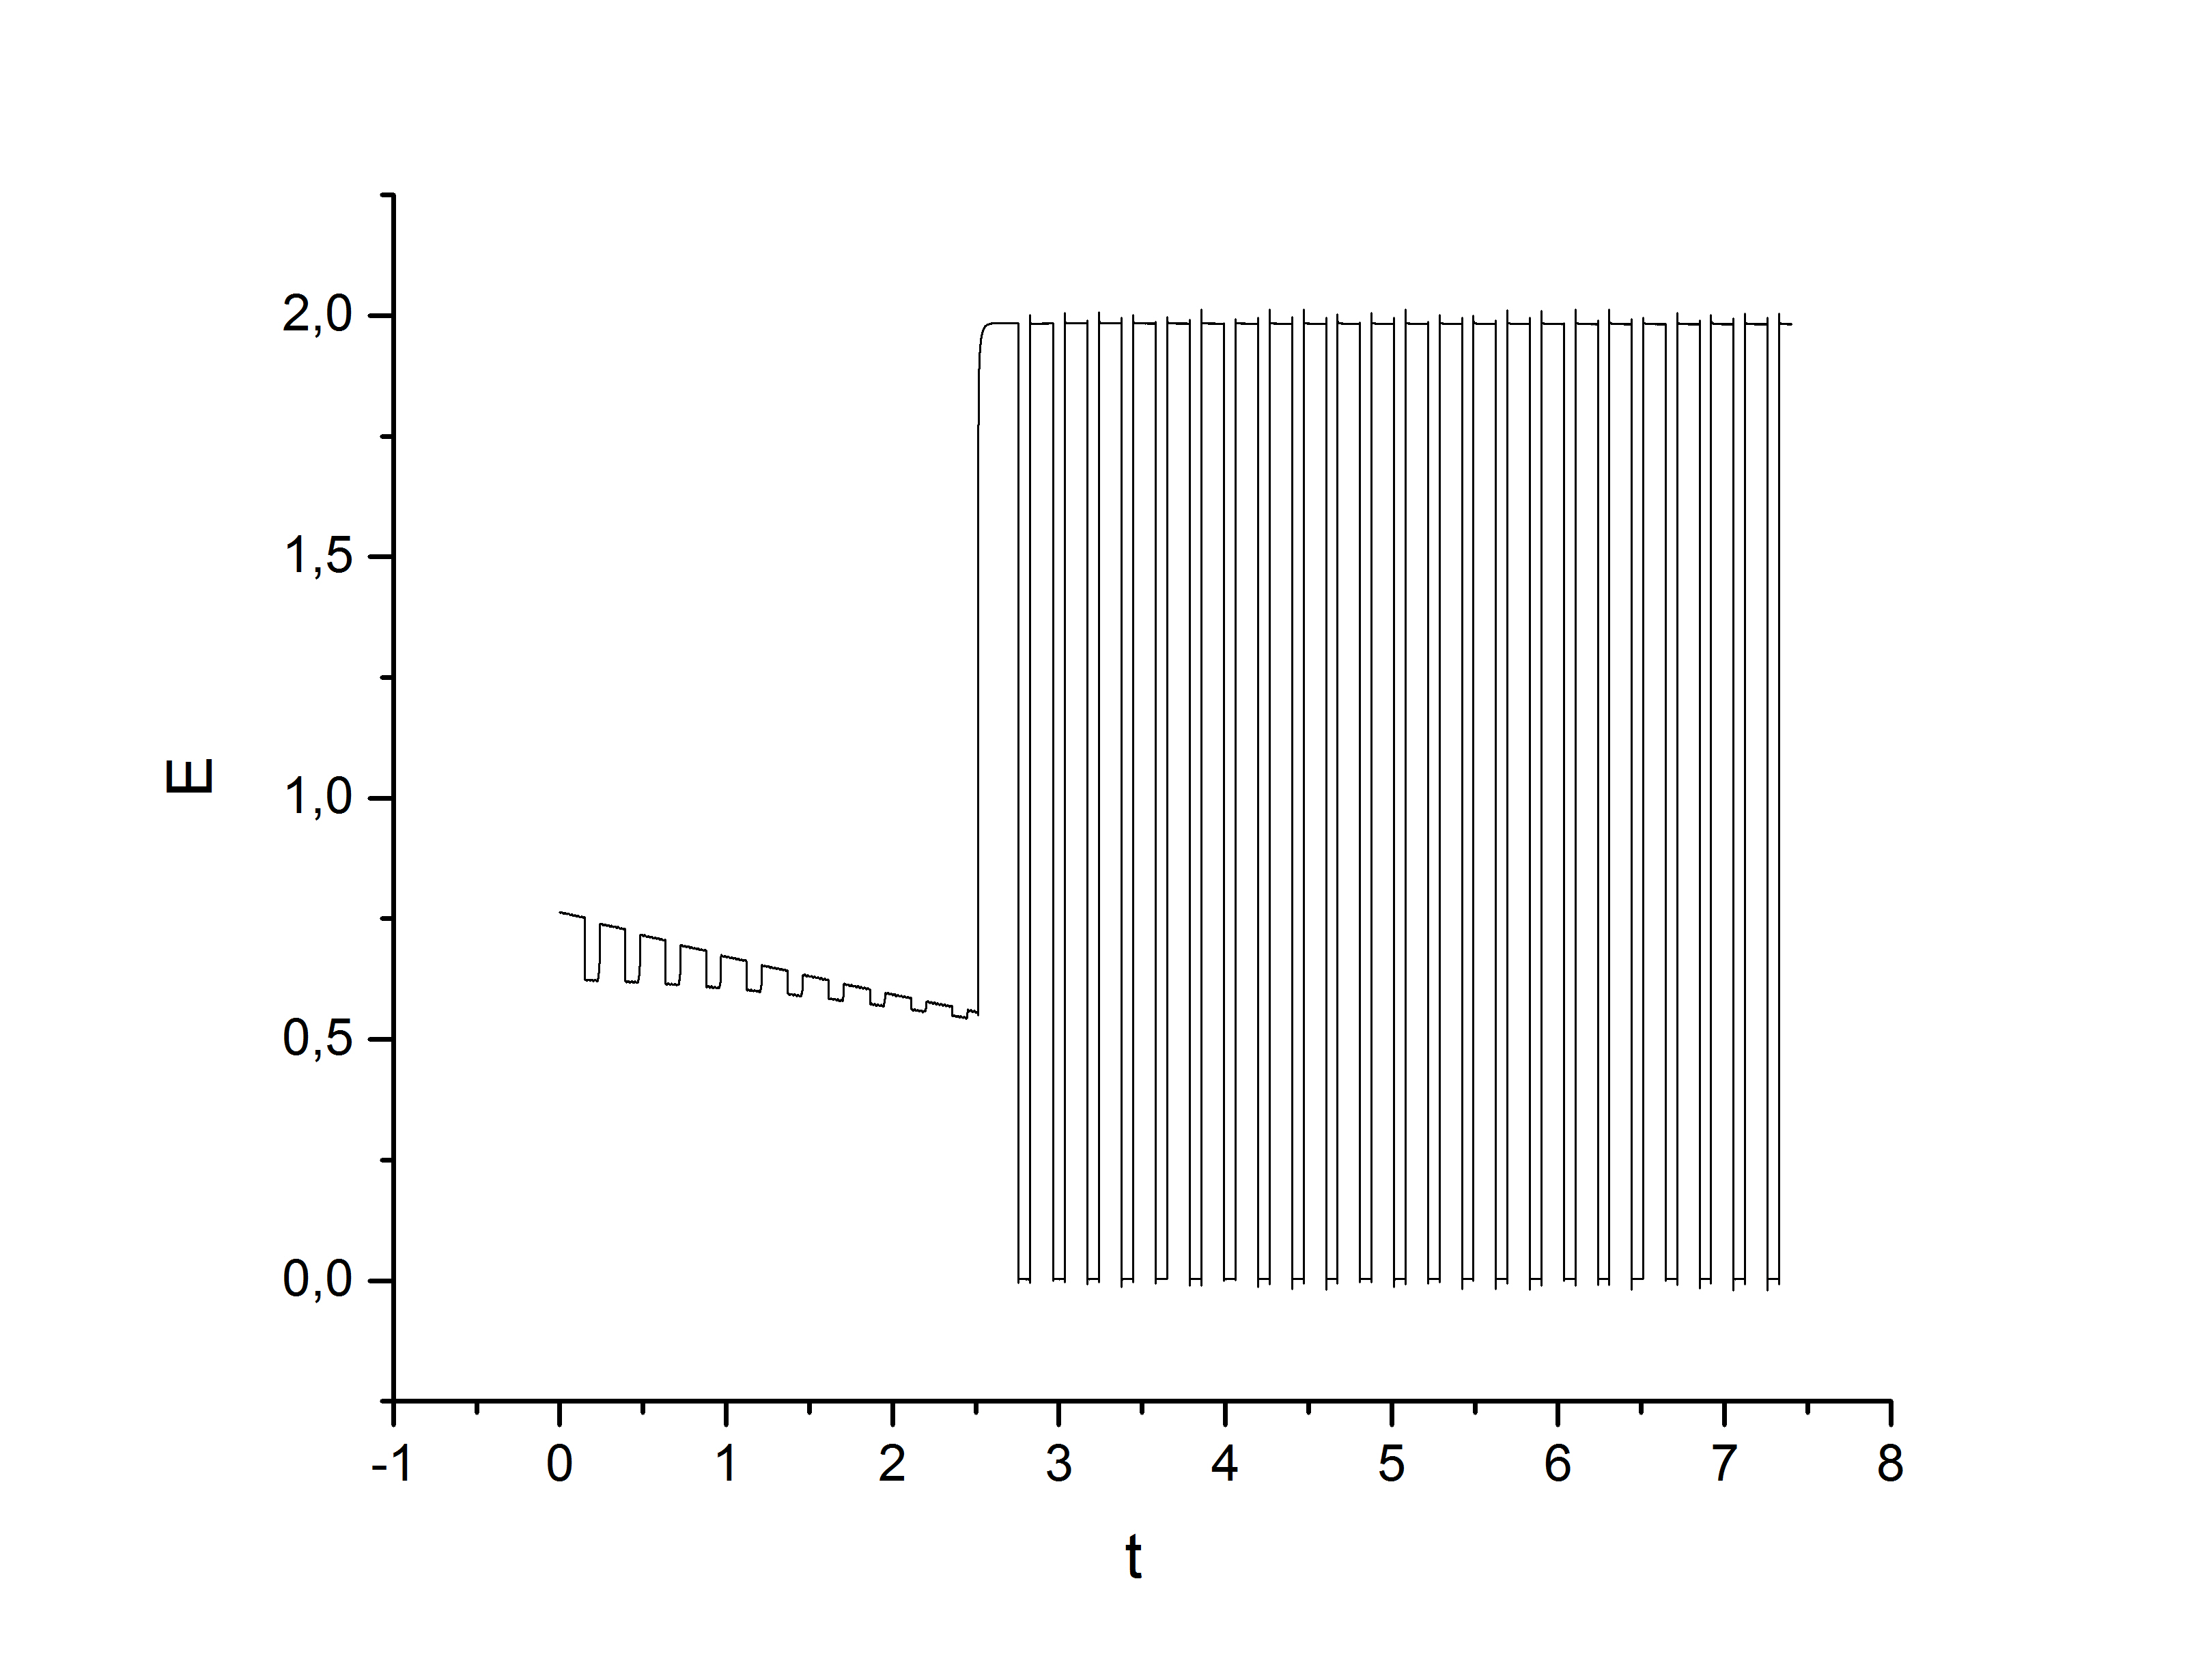
\includegraphics[width=0.8\textwidth]{img/square.jpg}
\caption{A "flip-flop" 2 V-os, 200 ms-os négyszöghullámra mért potenciál.}
\label{fig:square}
\end{figure}

\section{Kevert BZ makroelektróddal}
A Belouszov-Zsabotyinszkij reakció tanulmányozását a gyárilag előállított makroméretű elektródokkal kezdtem a mérés begyakorolása valamint Kőrös Endre eredményeinek \cite{noyes1972oscillations} reprodukálása végett. 
\begin{figure}[h]
\centering
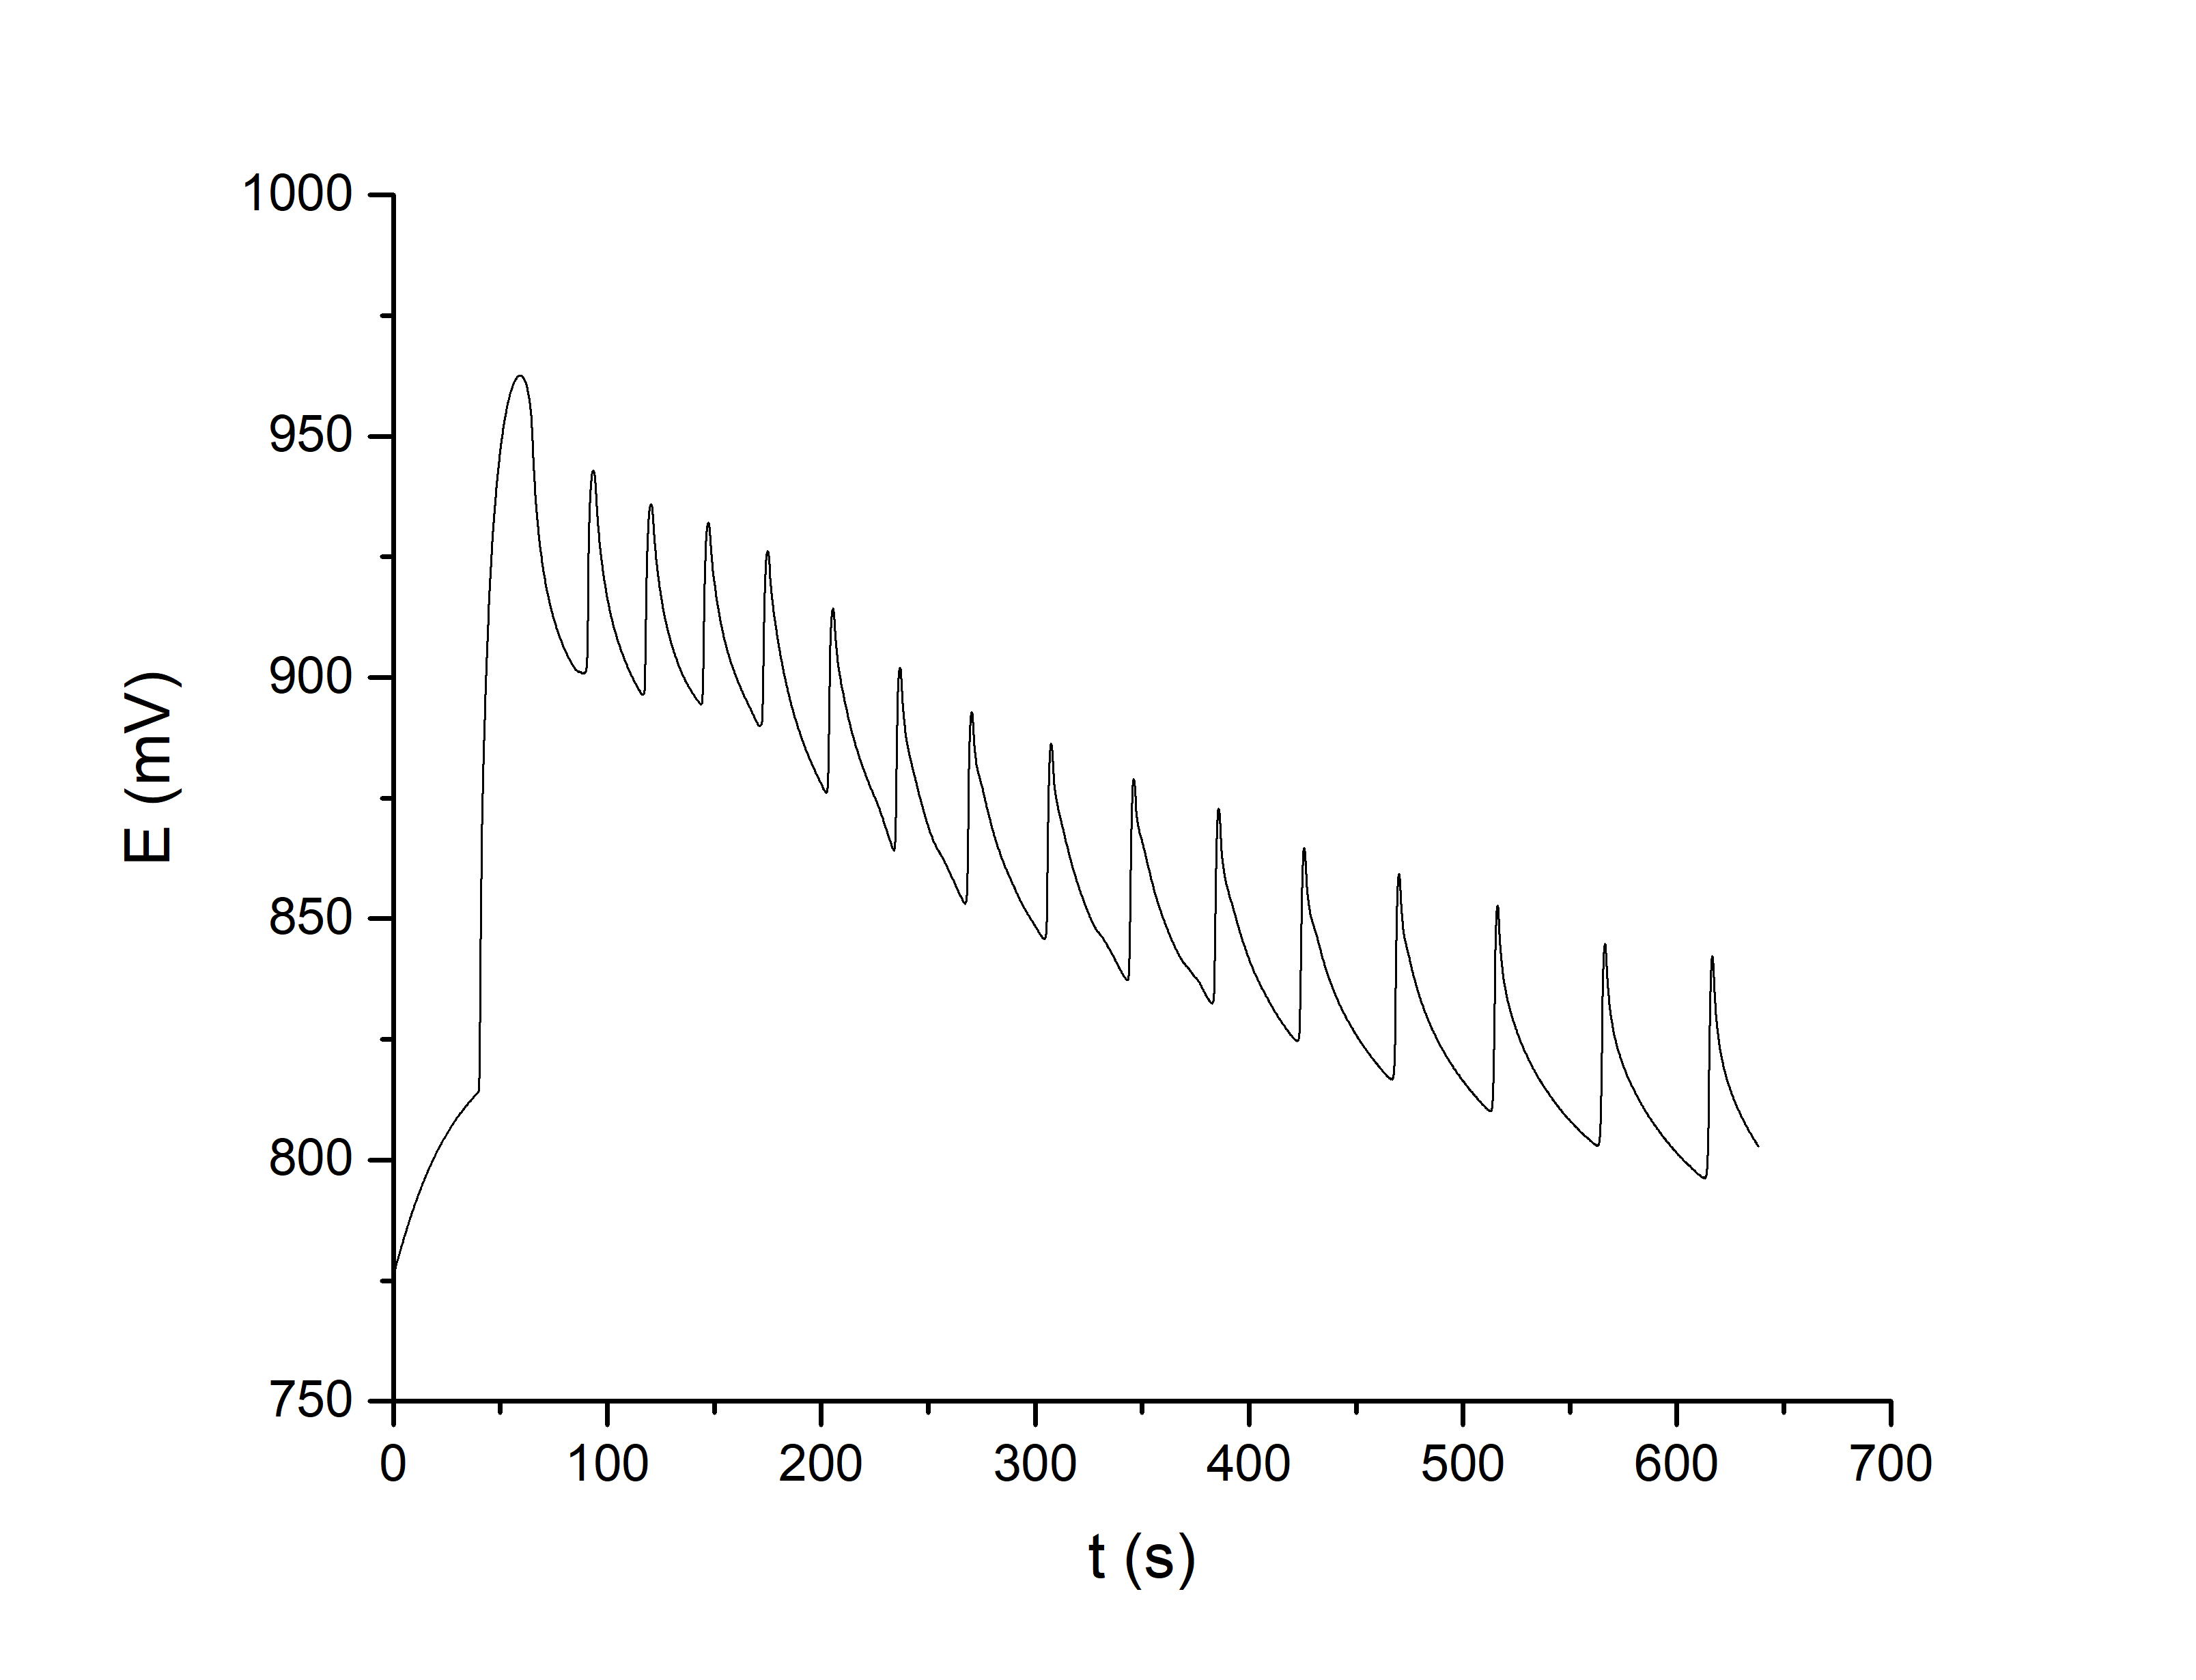
\includegraphics[width=0.8\textwidth]{img/makroelektrod.jpg}
\caption{Kevert BZ-reakció vizsgálata makroméretű platina elektróddal.}
\label{fig:makroelektrod}
\end{figure}
A \ref{fig:makroelektrod} ábrán látható, hogy a \ref{celkituzes} című bekezdés 1. pontjában megemlített Field, Noyes és Kőrös eredményeit \cite{noyes1972oscillations} sikeresen reprodukáltam. Továbbá látható a kevertetett oszcilláló reakció esetén a periódusidő az idő függvényében közel lineárisan csökken. 

\section{Kevert BZ mikroelektródokkal}

Az \ref{fig:platina_kevert} ábrán a \ref{celkituzes} című fejezet 3. pontjának megismétlése látható, azaz Nagy-Ungvárai és Hess munkáját sikerült reprodukálnom és az általam készített mikroelektródok alkalmazhatóságát bizonyítanom.

\begin{figure}[h]
\centering
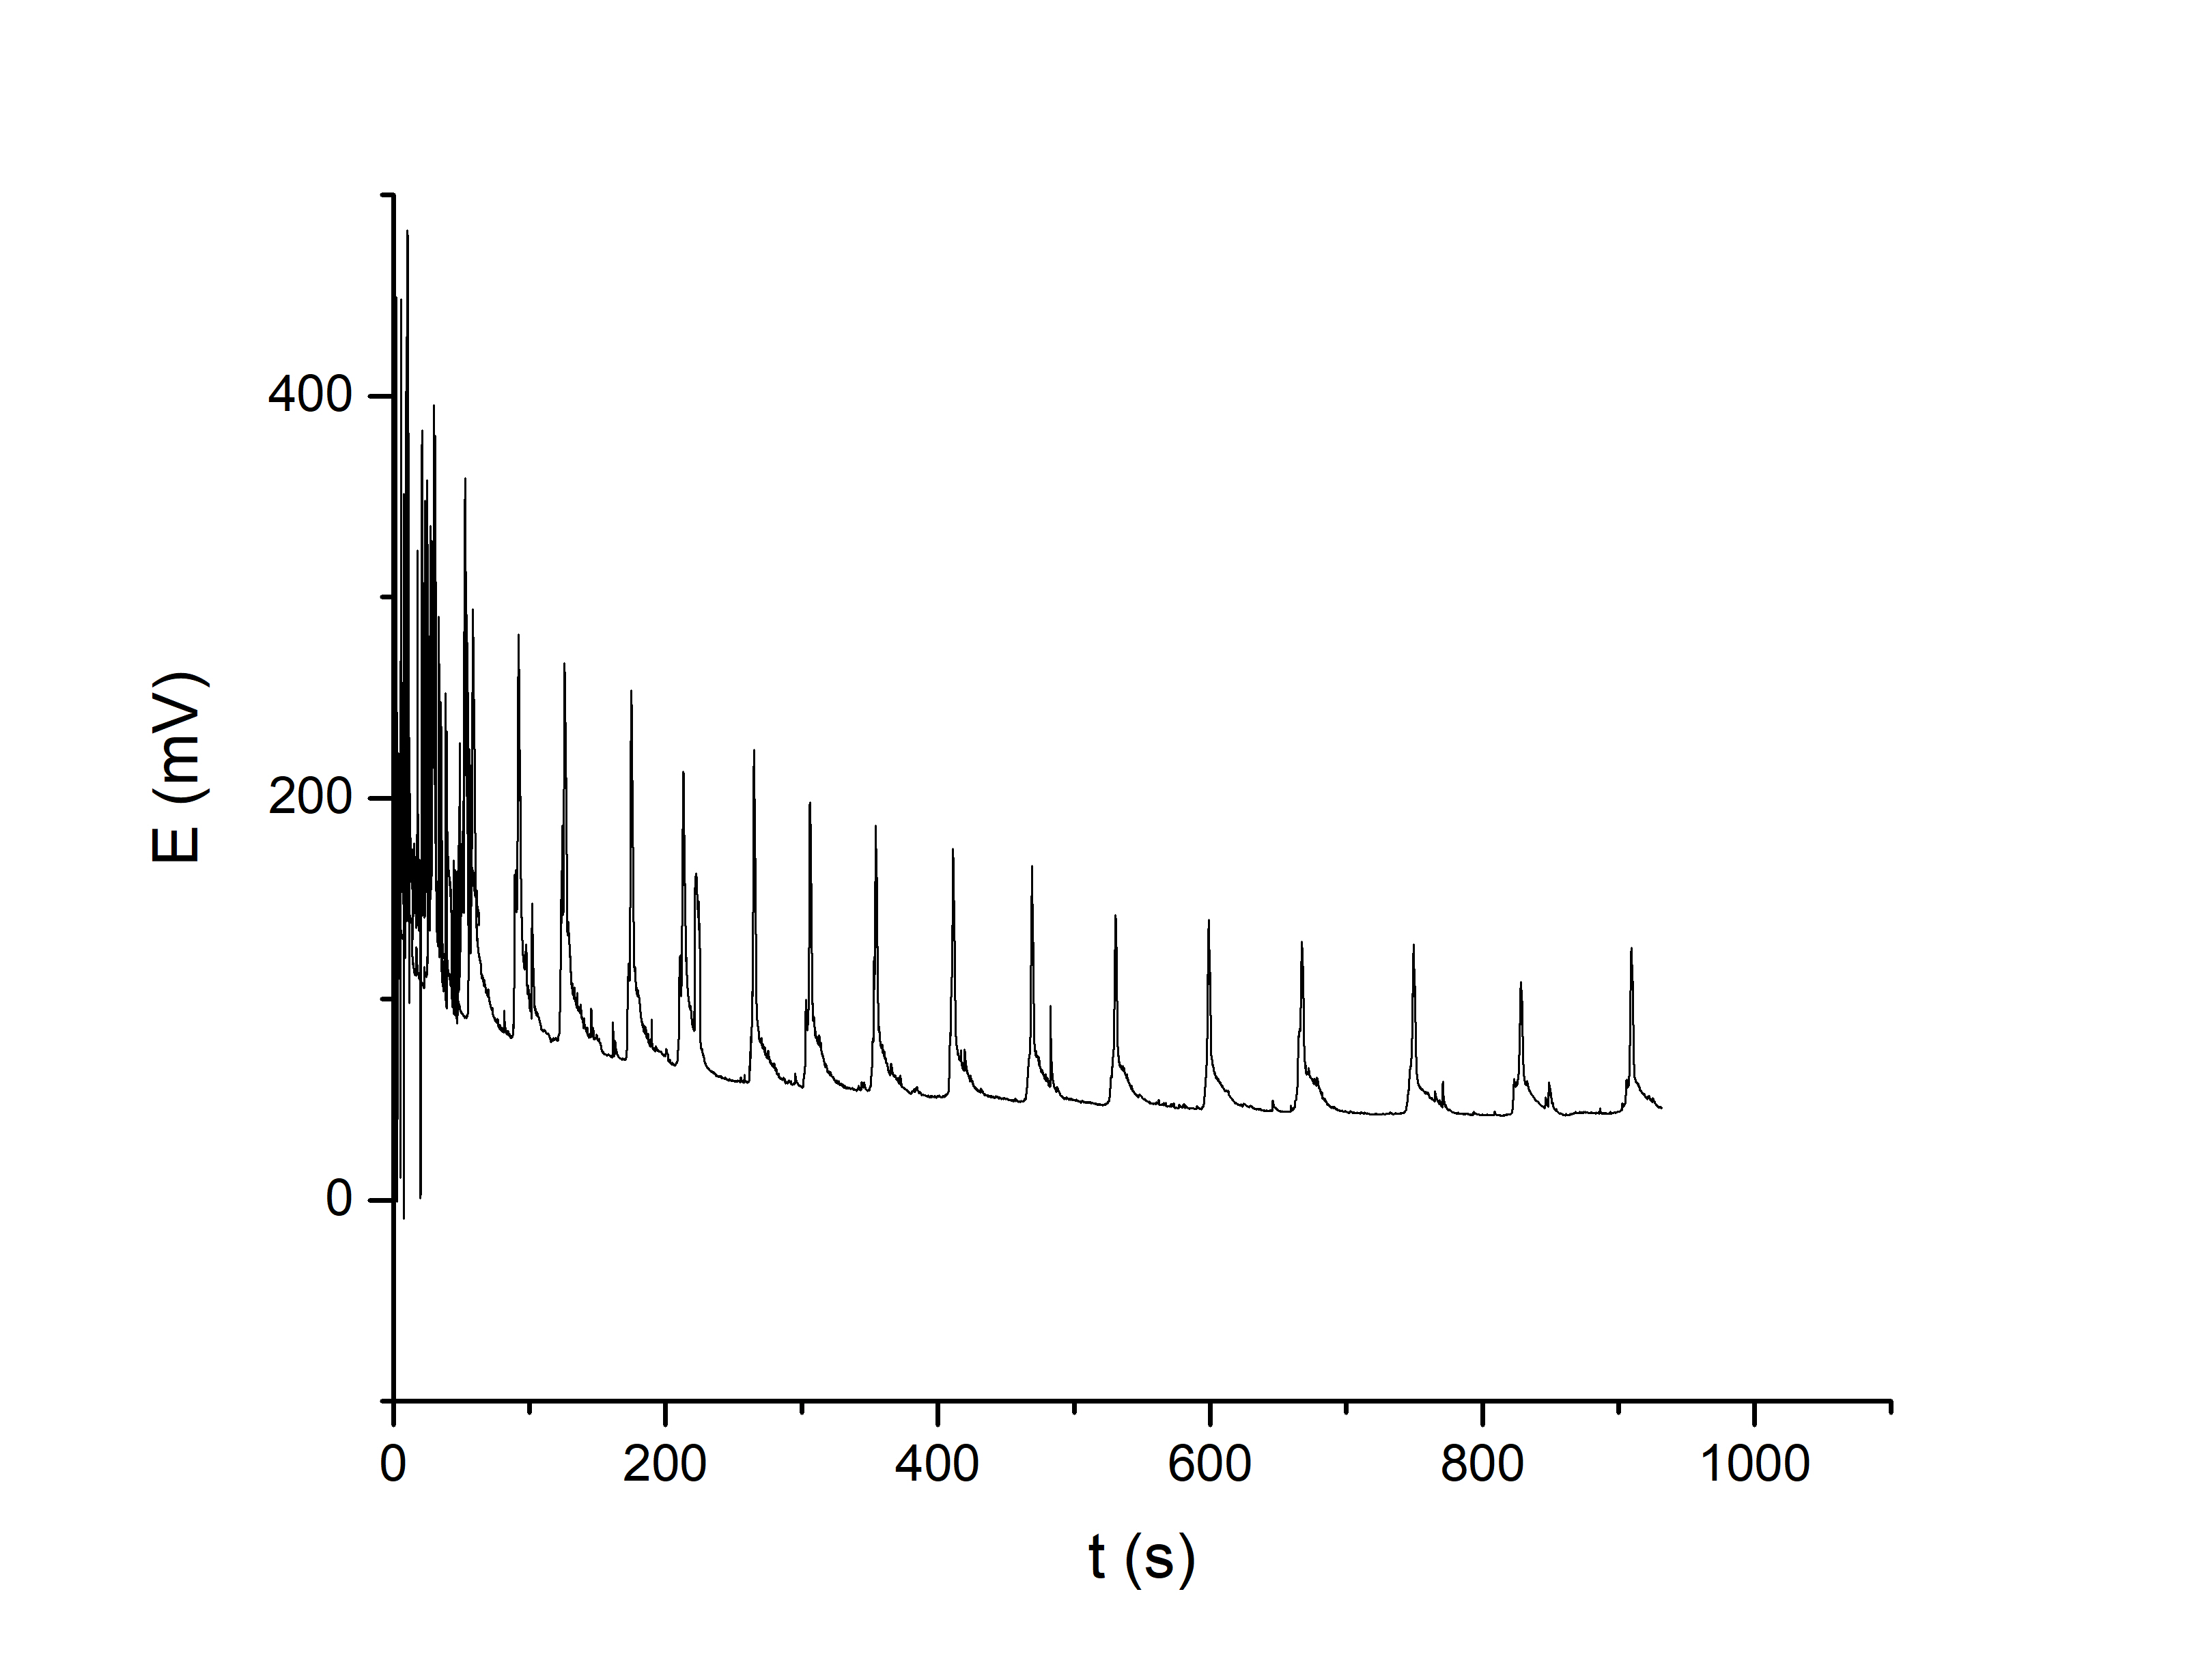
\includegraphics[width=0.8\textwidth]{img/platina_kevert.jpg}
\caption{Kevert BZ-reakció vizsgálata  platina mikroelektróddal.}
\label{fig:platina_kevert}
\end{figure}


\section{Keveretlen BZ mikroelektródokkal}
A könnyebben vizsgálható kevertetett reakció tanulmányozása után a keveretlen reakció tanulmányozására használtam fel az általam készített különböző potenciometriás mikroelektródokat.
\begin{figure}[h]
\centering
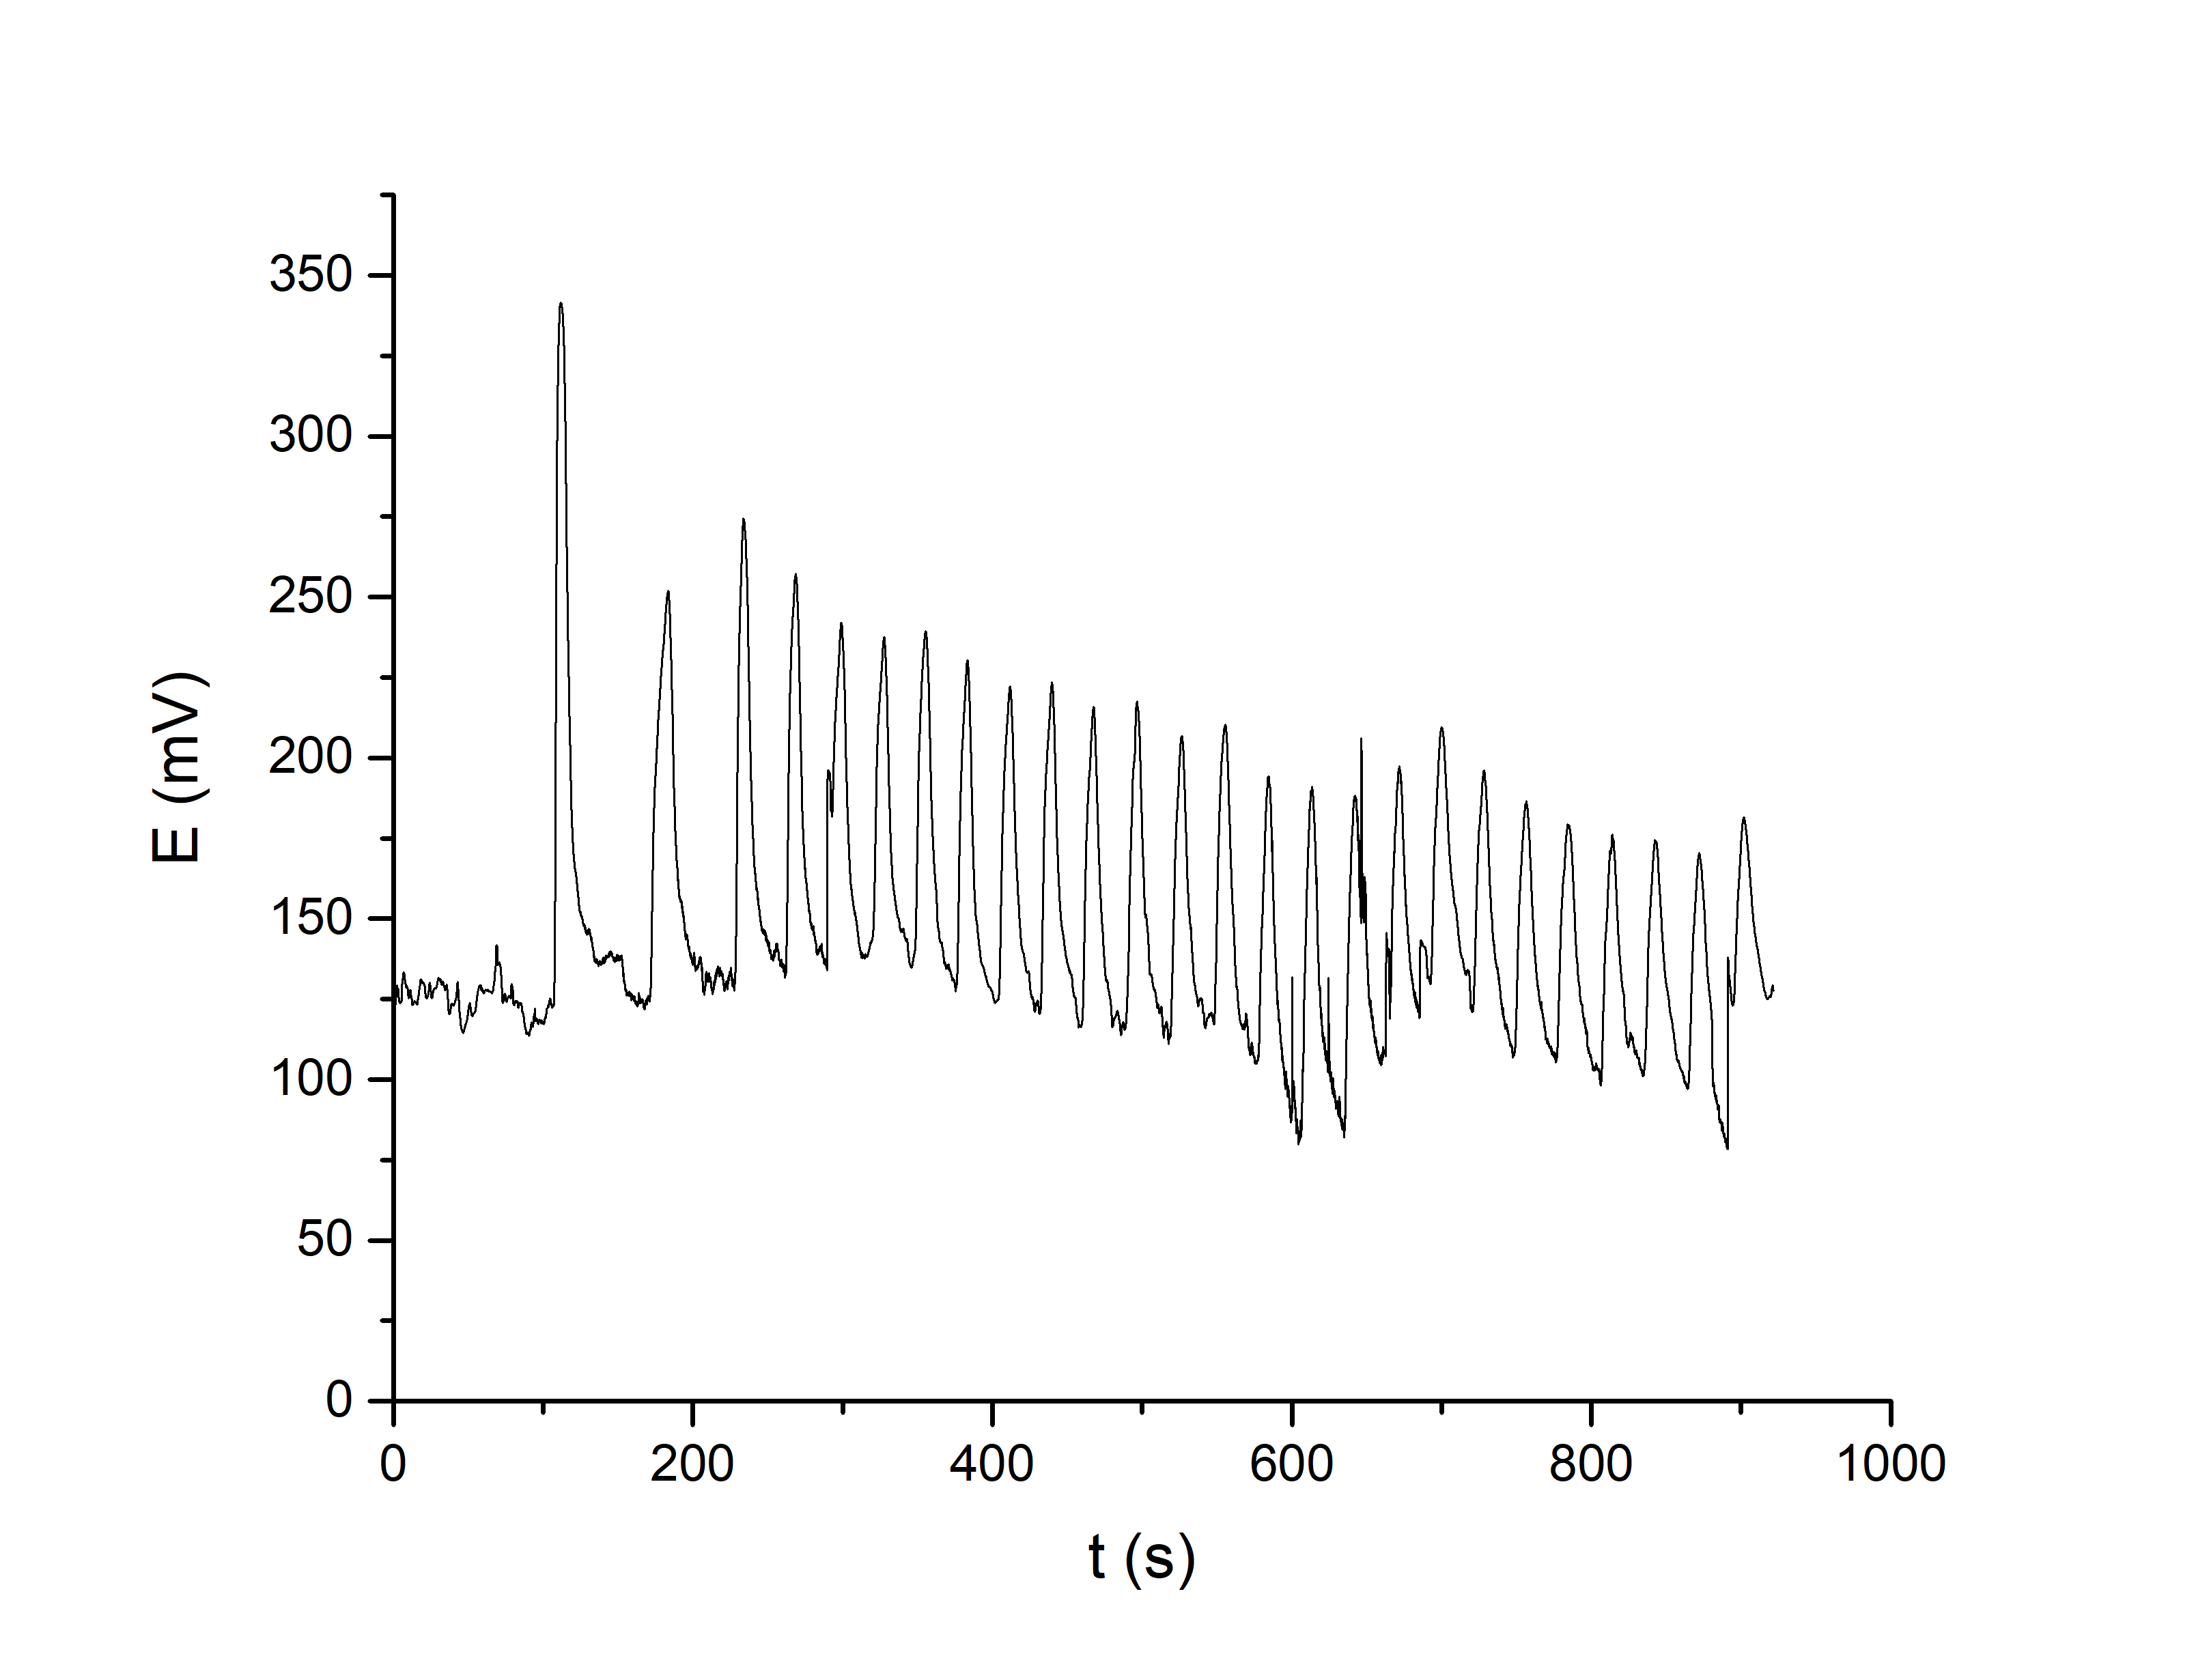
\includegraphics[width=0.8\textwidth]{img/platina_keveretlen.jpg}
\caption{Redoxpotenciál vizsgálata keveretlen BZ-reakcióban, platina mikroelektróddal.}
\label{fig:platina_keveretlen}
\end{figure}

\section{Kevert és keveretlen BZ vizsgálata}
\subsection{Platina elektród}
A Belouszov-Zsabotyinszkij reakció tanulmányozását a gyárilag előállított makroméretű elektródokkal kezdtem a mérés begyakorolása valamint Kőrös Endre eredményeinek \cite{noyes1972oscillations} reprodukálása végett. Miután begyakoroltam a módszert, a saját készítésű elektróddal kezdtem el vizsgálni a már említett reakciót. A vizsgálatok során először kevertetve tanulmányoztam az oldatot, a kevertetést mágneses keverő segítségével valósítottam meg. A kevertetett reakció többszöri vizsgálata után kevertetést nem használva vizsgáltam a rendszert.
\begin{figure}[h]
\centering
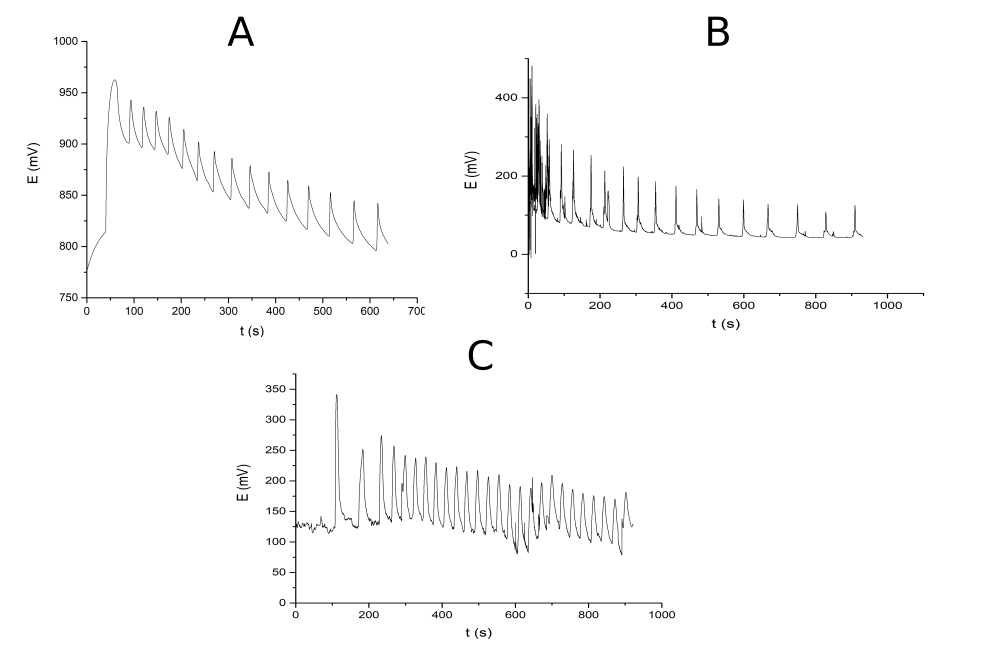
\includegraphics[width=1\textwidth]{img/platina_meres.png}
\caption{A BZ-reakció tanulmányozása platina elektródokkal.}
\label{fig:platina_meres}
\end{figure}
A \ref{fig:platina_meres} ábrán látható (A) kép a kevert rendszer vizsgálata makroméretű platina elektróddal. A vizsgálatból megfigyelhető, hogy a kevertett reakció esetében a periódusidő az idő függvényében közel lineárisan csökken. A (B) képen az adott kevert reakció tanulmányozása mikroméretű platina elektróddal.A (C) ábrán az előző alkalommal vizsgált rendszer keverés nélkül. A vizsgálatok során mértem a platina elektródokon kialakult potenciál a referencia elektródhoz (Ag/AgCl) képest. A \ref{celkituzes} című bekezdés 1. pontjában megemlített Field, Noyes és Kőrös eredményeit \cite{noyes1972oscillations} sikeresen reprodukáltam.  

%\section{Kevert BZ mikroelektródokkal}

%Az \ref{fig:platina_kevert} ábrán a \ref{celkituzes} című fejezet 3. pontjának megismétlése látható, azaz Nagy-Ungvárai és Hess munkáját sikerült reprodukálnom és az általam készített mikroelektródok alkalmazhatóságát bizonyítanom.

%\begin{figure}[h]
%\centering
%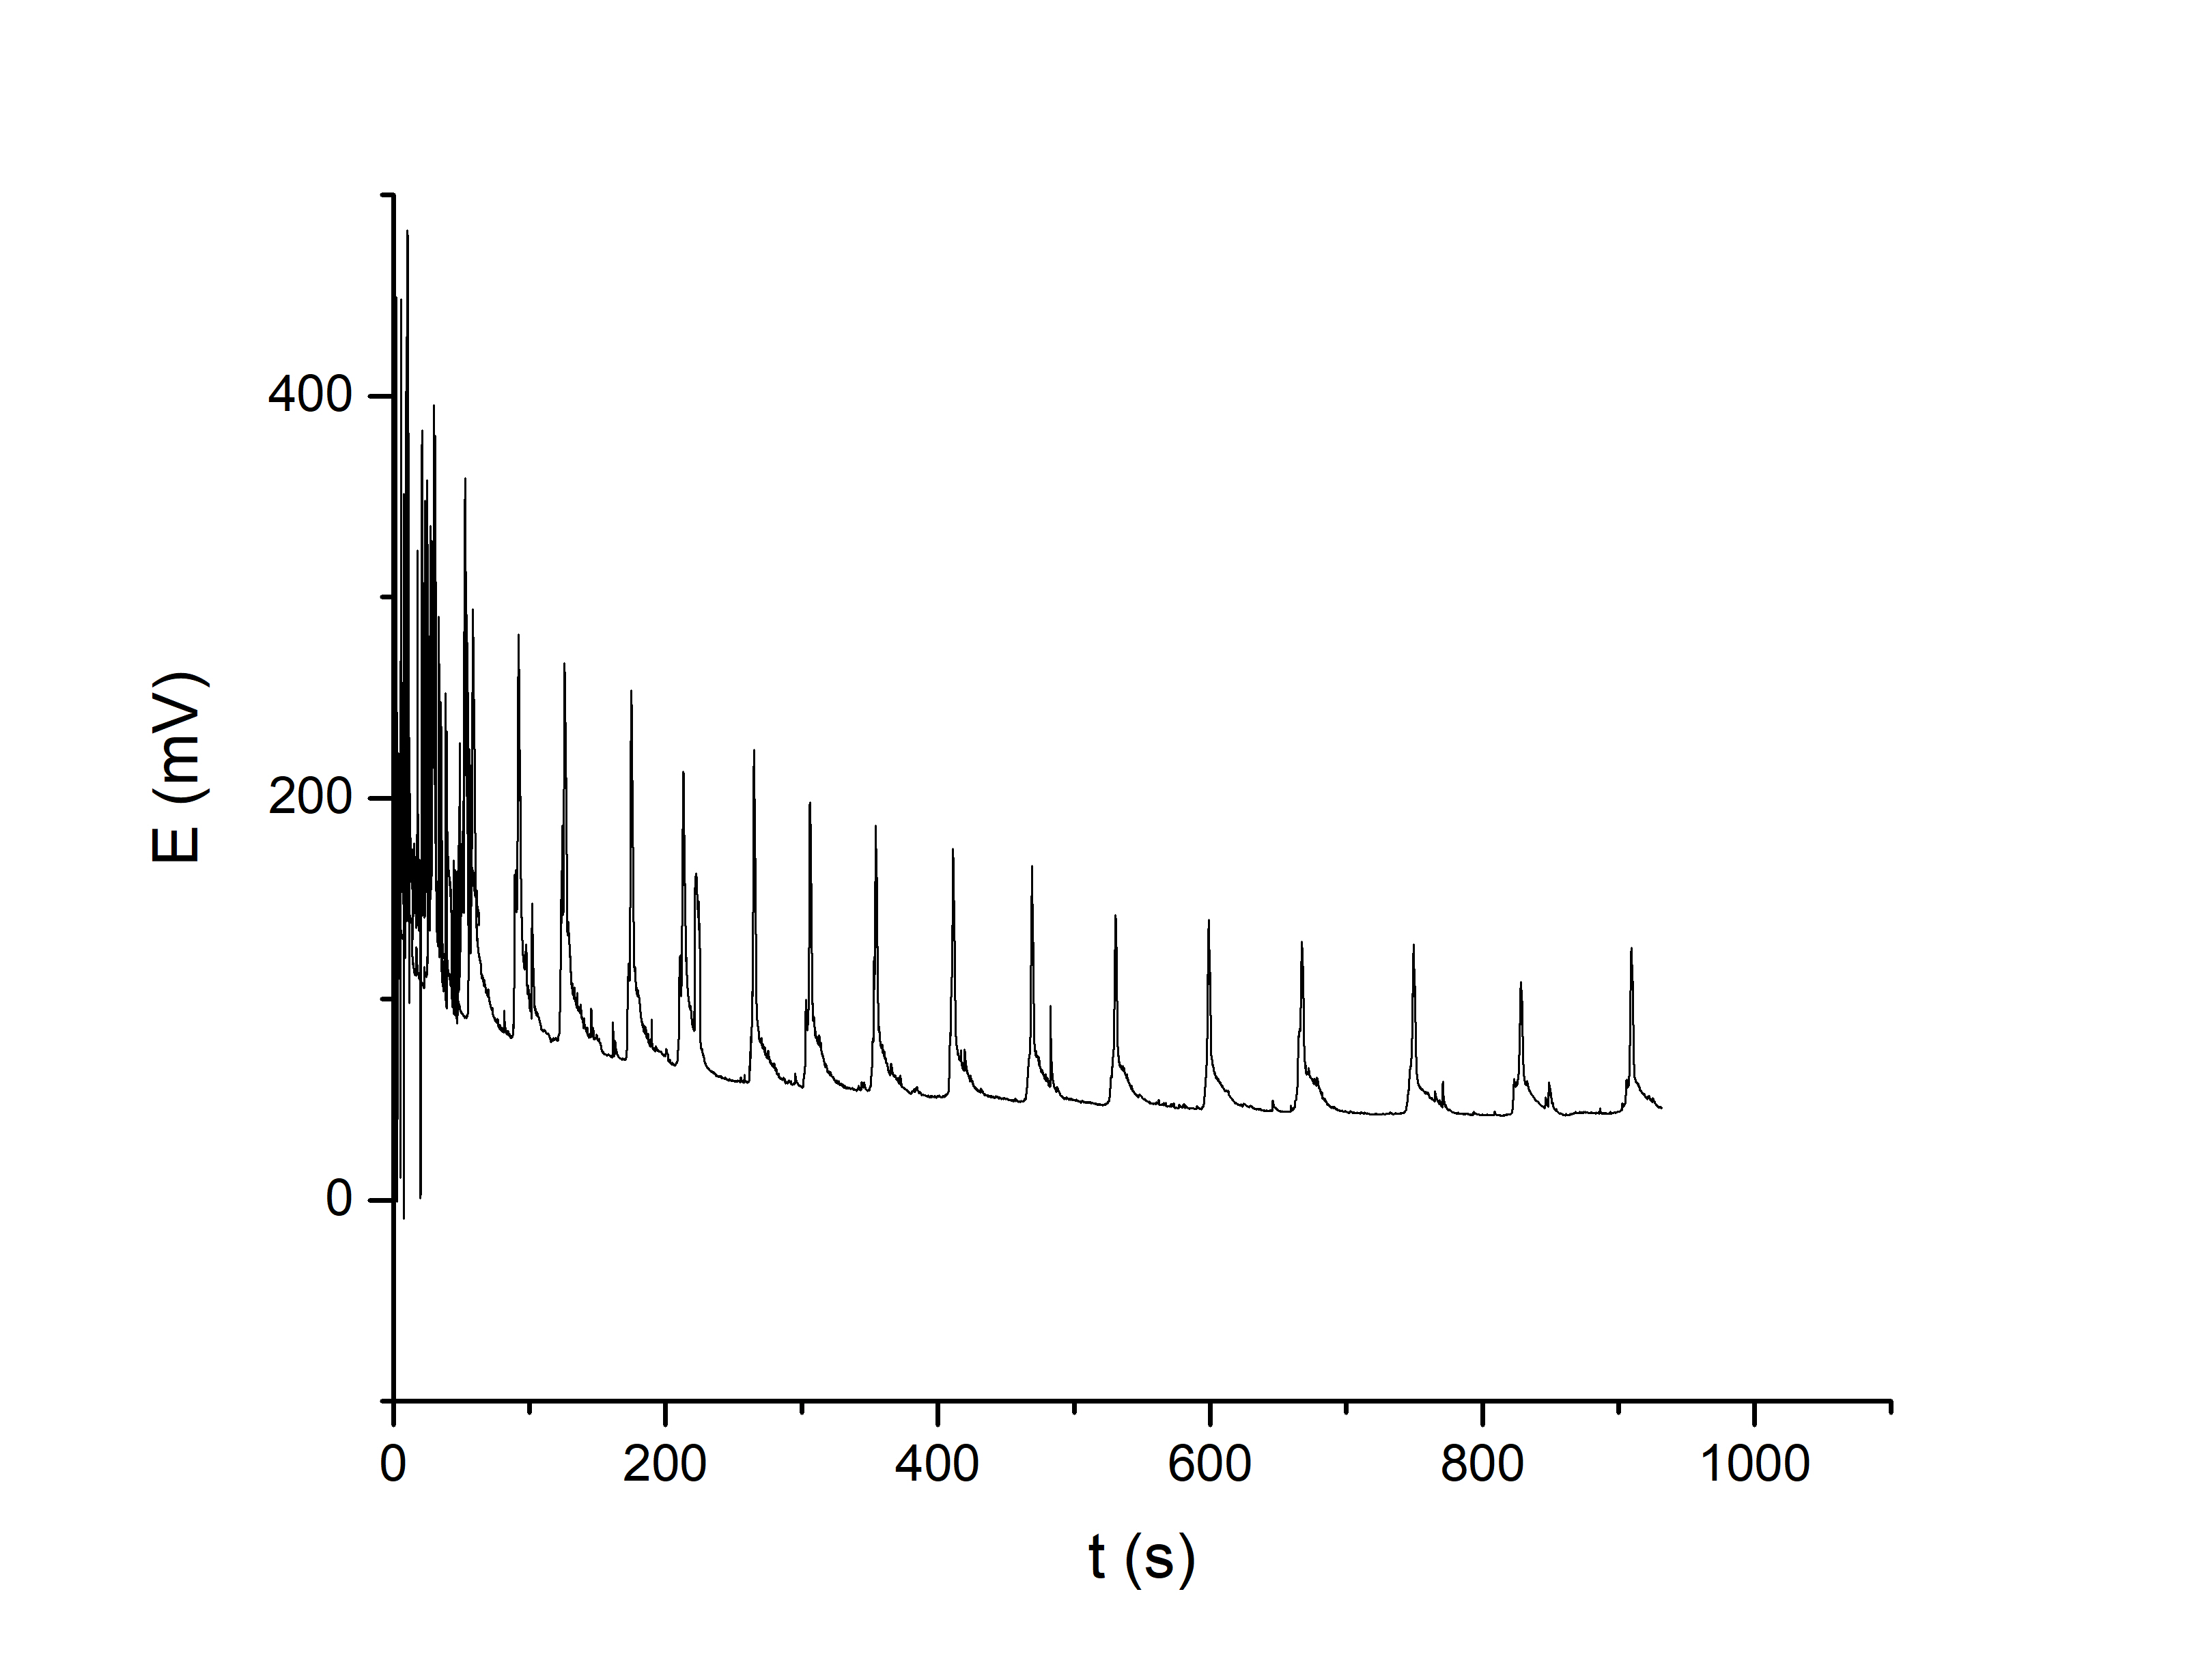
\includegraphics[width=0.8\textwidth]{img/platina_kevert.jpg}
%\caption{Kevert BZ-reakció vizsgálata  platina mikroelektróddal.}
%\label{fig:platina_kevert}
%\end{figure}


%\section{Keveretlen BZ mikroelektródokkal}
%A könnyebben vizsgálható kevertetett reakció tanulmányozása után a keveretlen reakció tanulmányozására használtam fel az általam készített különböző potenciometriás mikroelektródokat.
%\begin{figure}[h]
%\centering
%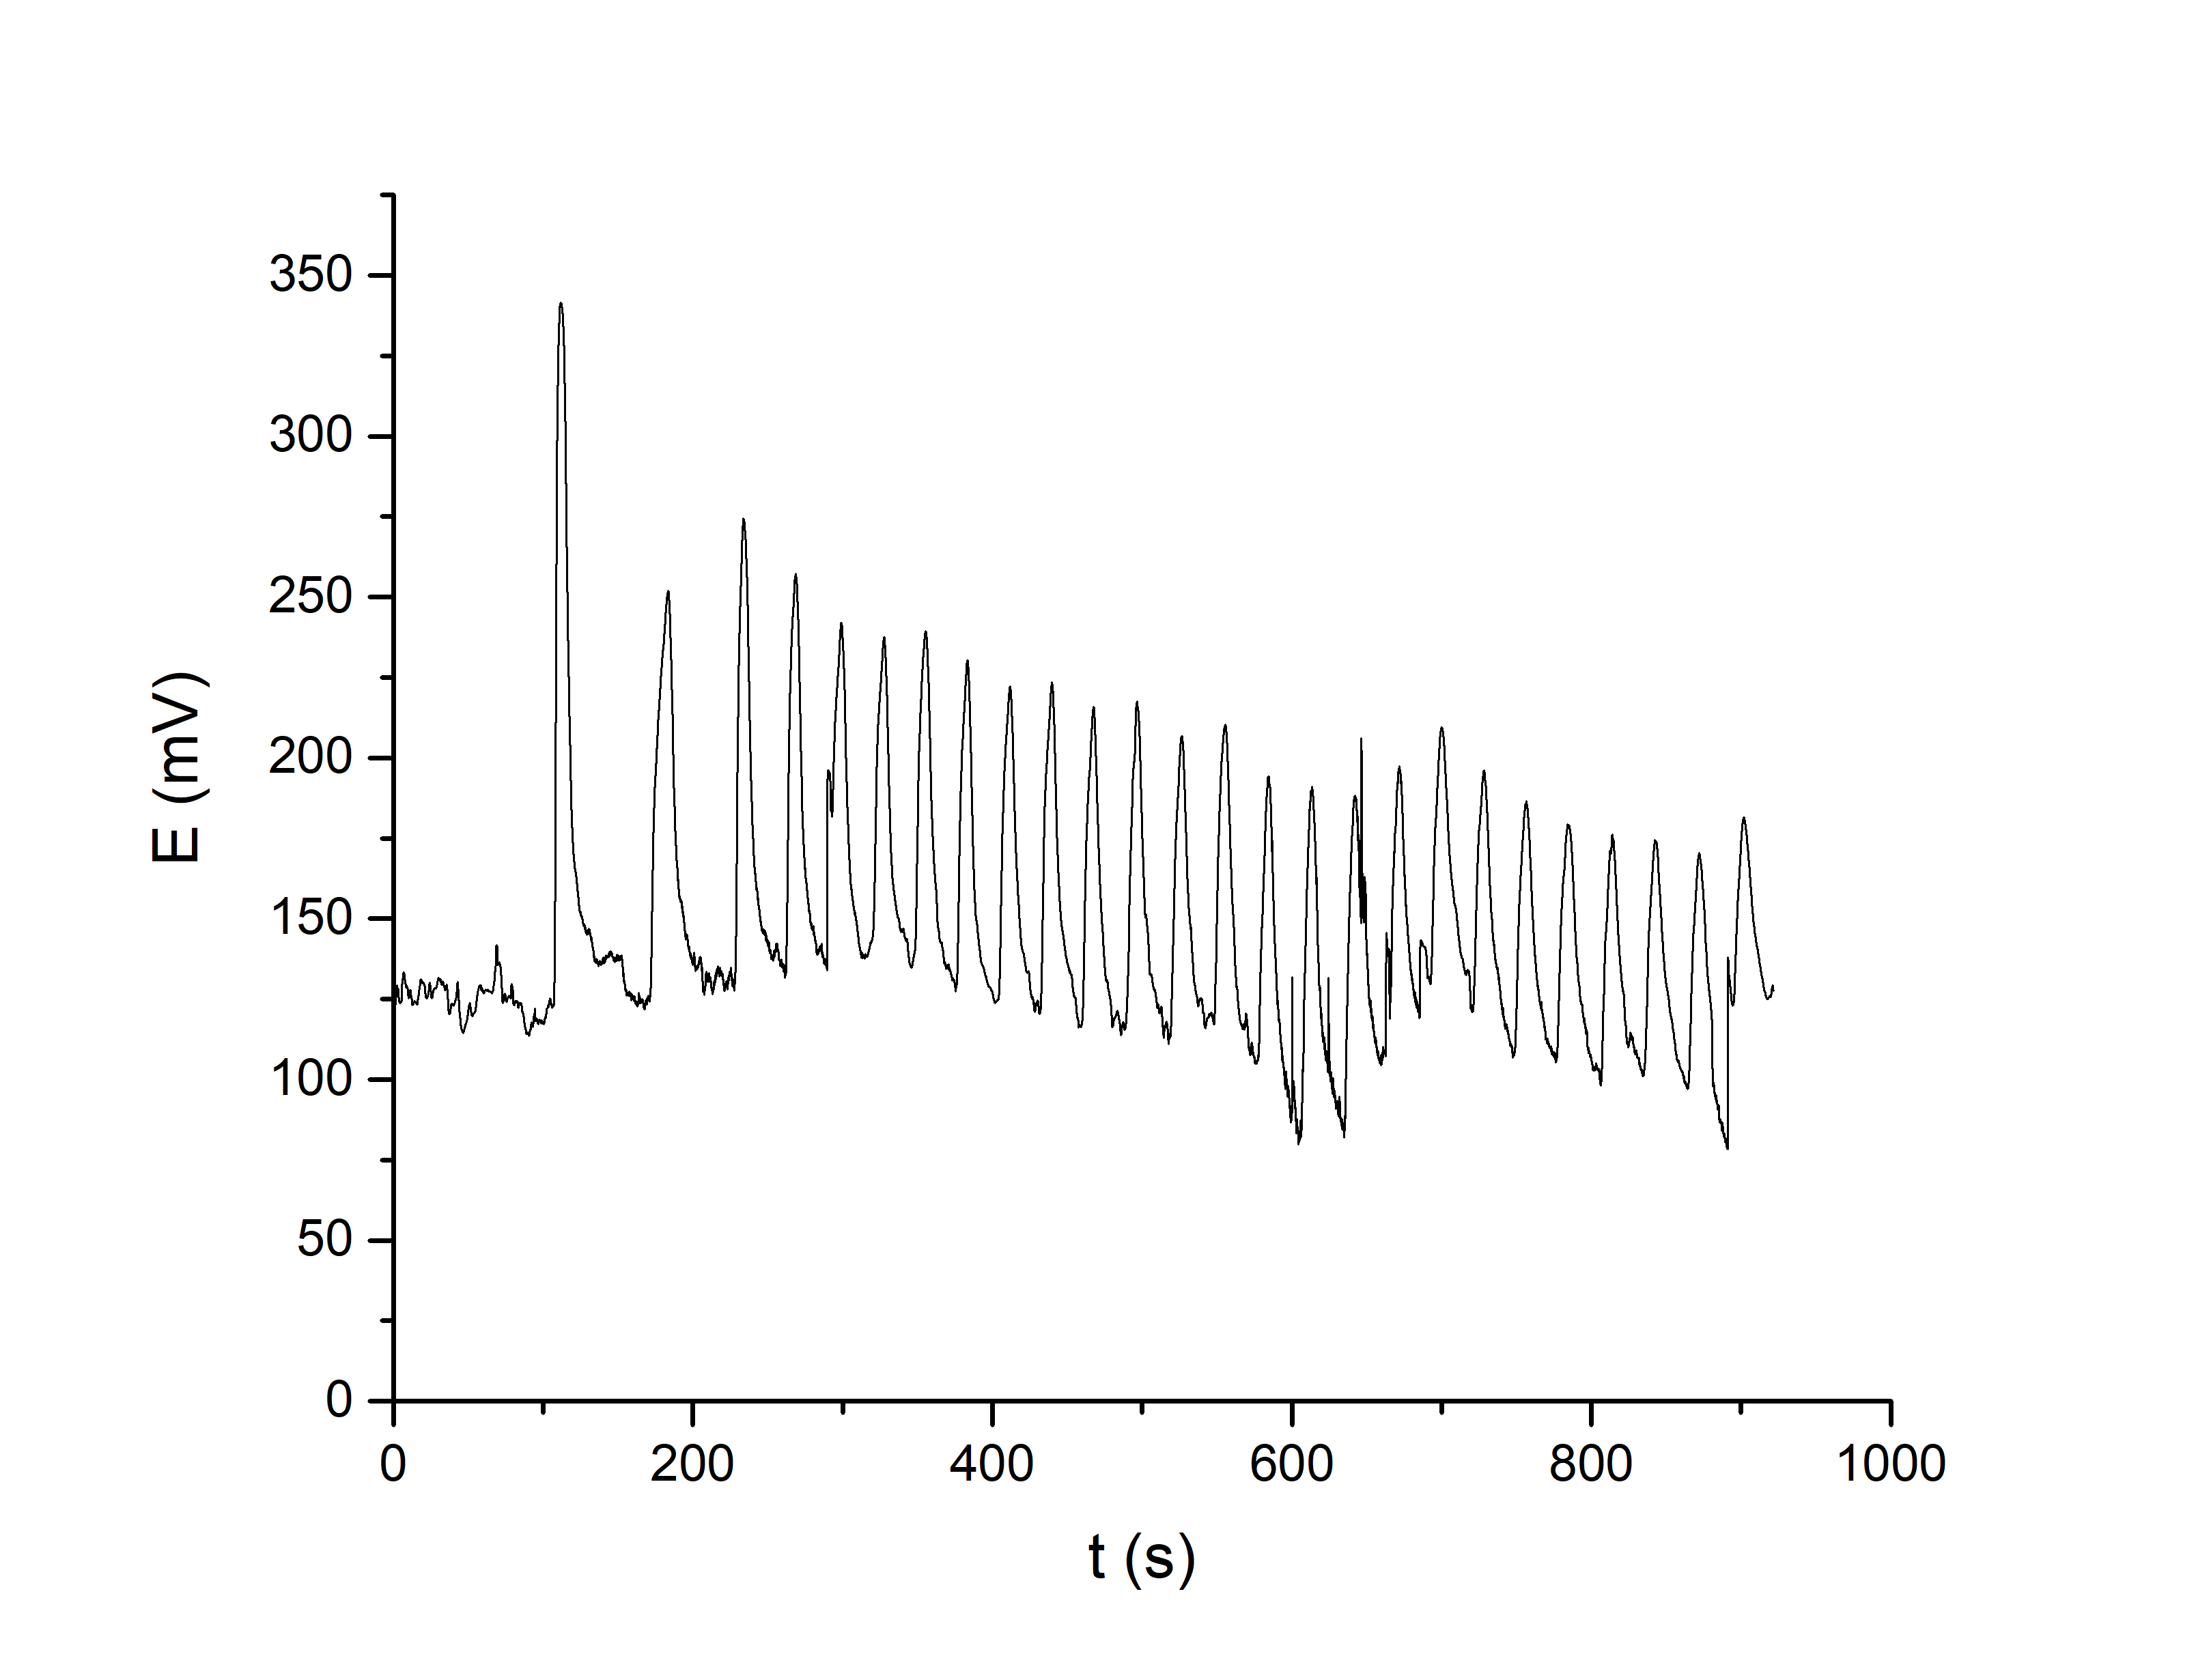
\includegraphics[width=0.8\textwidth]{img/platina_keveretlen.jpg}
%\caption{Redoxpotenciál vizsgálata keveretlen BZ-reakcióban, platina mikroelektróddal.}
%\label{fig:platina_keveretlen}
%\end{figure}

%\begin{figure}[h]
%\centering
%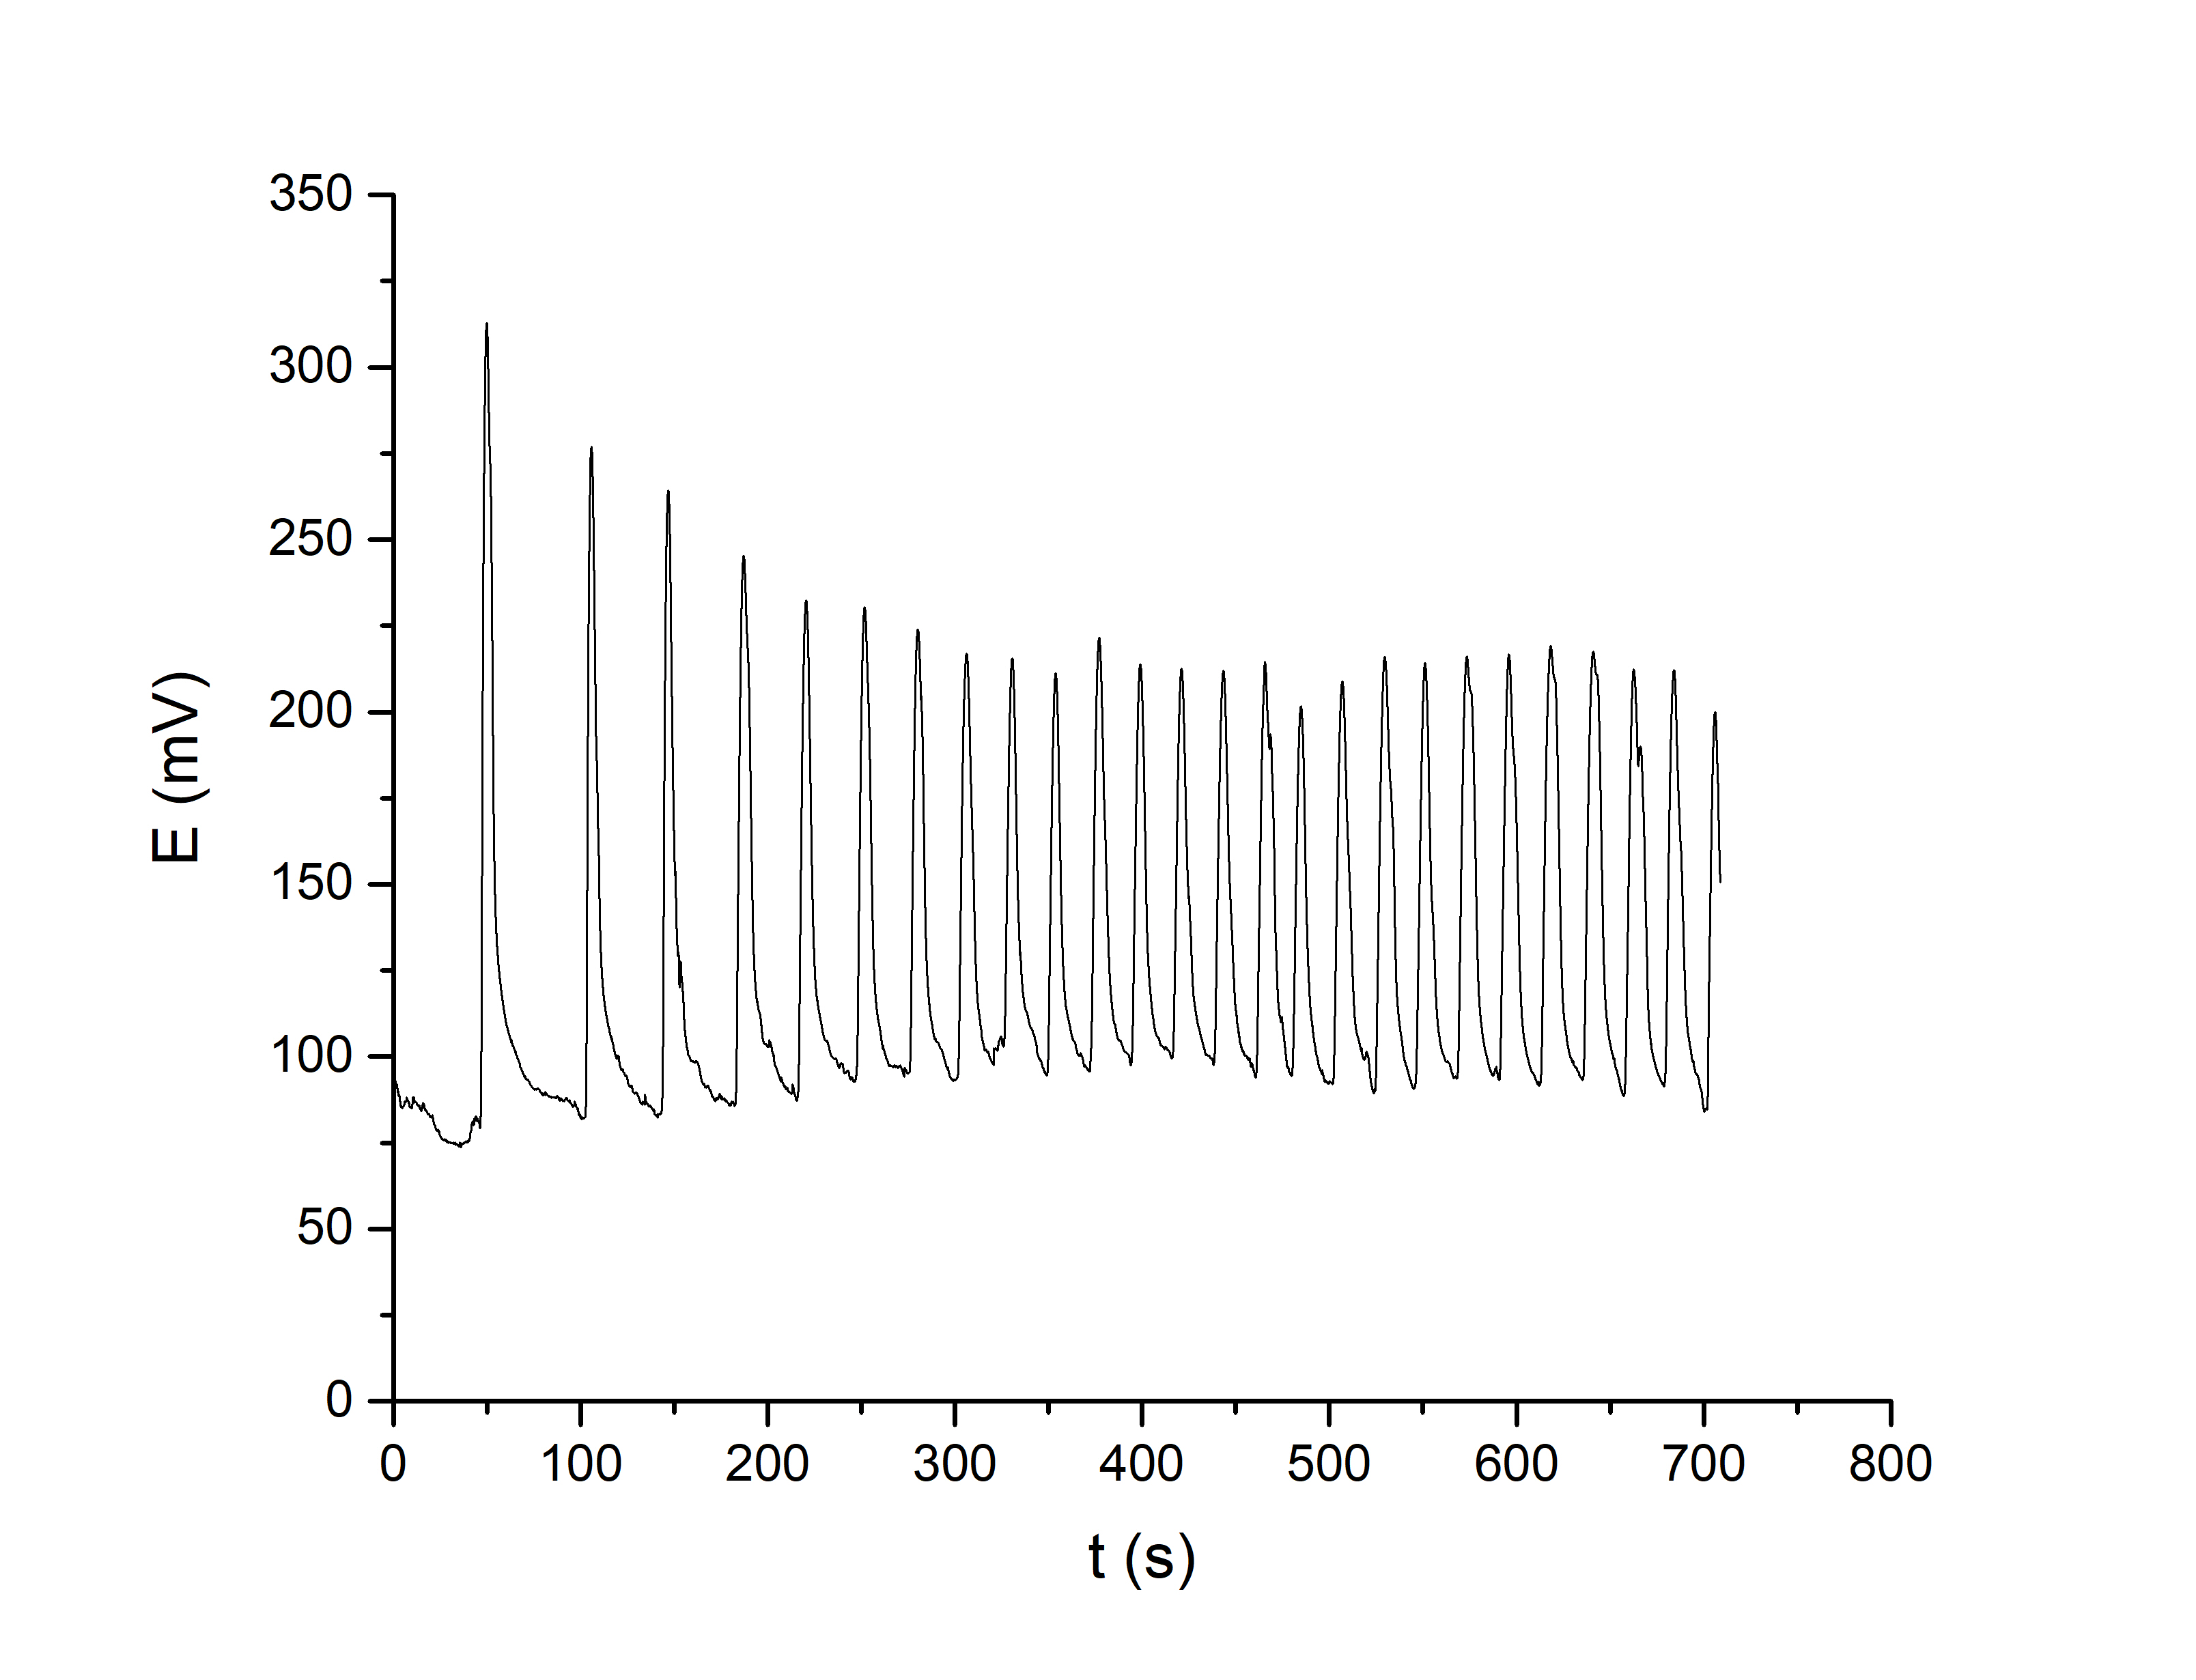
\includegraphics[width=0.8\textwidth]{img/szen33_keveretlen.jpg}
%\caption{Redoxpotenciál tanulmányozása keveretlen BZ-reakcióban 33 $\upmu$m-es szén mikroelektróddal.}
%\label{fig:szen33_keveretlen}
%\end{figure}

\section{Pontszerű mérés}
A keveretlen reakció elektrokémiai tanulmányozását optikai módszer felhasználásával tovább bővítettem. Az előző pontban végzett vizsgálatok alapján és a későbbiekben előkerülő miniatűrizálás érdekében szén mikroelektródokkal folyattam a vizsgálatokat. Az elektrokémiai jelet optikai képpel kombináltam,ennek eredményét  mutatom be ezen a pontban. Az optikai képet az \emph{"Optikai tér-idő kép szerkeztése} című fejezetben leírt módszer alapján készítettem.

\section{Pontszerű mérés keveretlen BZ}
A keveretlen reakció elektrokémiai tanulmányozását optikai módszer felhasználásával tovább bővítettem. Az előző pontban végzett vizsgálatok alapján és a későbbiekben előkerülő miniatűrizálás érdekében szén mikroelektródokkal folyattam a vizsgálatokat. Az elektrokémiai jelet optikai képpel kombináltam,ennek eredményét  mutatom be ezen a pontban.
\begin{figure}[h]
\centering
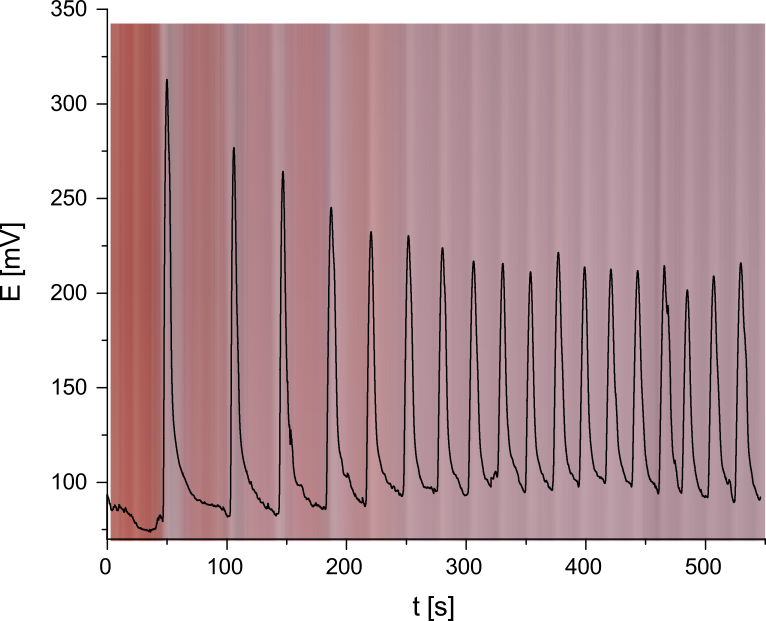
\includegraphics[width=0.8\textwidth]{img/pontszerumeres.png}
\caption{Elektrokémiai kép egy pontban.}
\label{fig:pontszerumeres}
\end{figure}

A \ref{fig:pontszerumeres} ábrán látható az optikai képhez az elektródpotenciált rendelve. A képen a kék szín az oxidált, a piros szín a redukált formához rendelhető.

\section{PEKM}
Az elektrokémiai és optikai módszert tovább gondolva kezdtem meg a PEKM alkalmazását, amely alapján elektrokémiai és optikai tér idő képet kaptam, ezeknek a képeknek a kombinálását mutatom be ebben a pontban. A két módszer kombinálásának előnye, hogy térbeli kémiai információt kapunk az adott felületről.
A PEKM használatát a 33 $\upmu$m átmérőjű szén-mikroelektróddal próbáltam eleinte megvalósítani, de ez "túl vastagnak" bizonyult. Finomítani kellett az elektródtesten, ugyanis nagy konvektív hatása van a pásztázás közben (szemmel látható kavarodást okoz a reakcióelegyben), ami a "nagy" átmérőből fakad. Ennek kiküszöbölésére egy 7 $\upmu$m átmérőjű szén-mikroelektródot alkalmaztam, amely során nem lép fel szemmel látható konvekció, vagyis a fellépő zavarást a rendszer diffúzió által ellensúlyozni tudja. Szemmel láthatóan kiküszöbölésre került az elektród által okozott konvekció, ugyanis a hullámok a reakciótér faláig zavaratlan formában haladtak tovább. Ez a  vizsgálat látható a \ref{fig:secmkep} ábrán.
\begin{figure}[h]
\centering
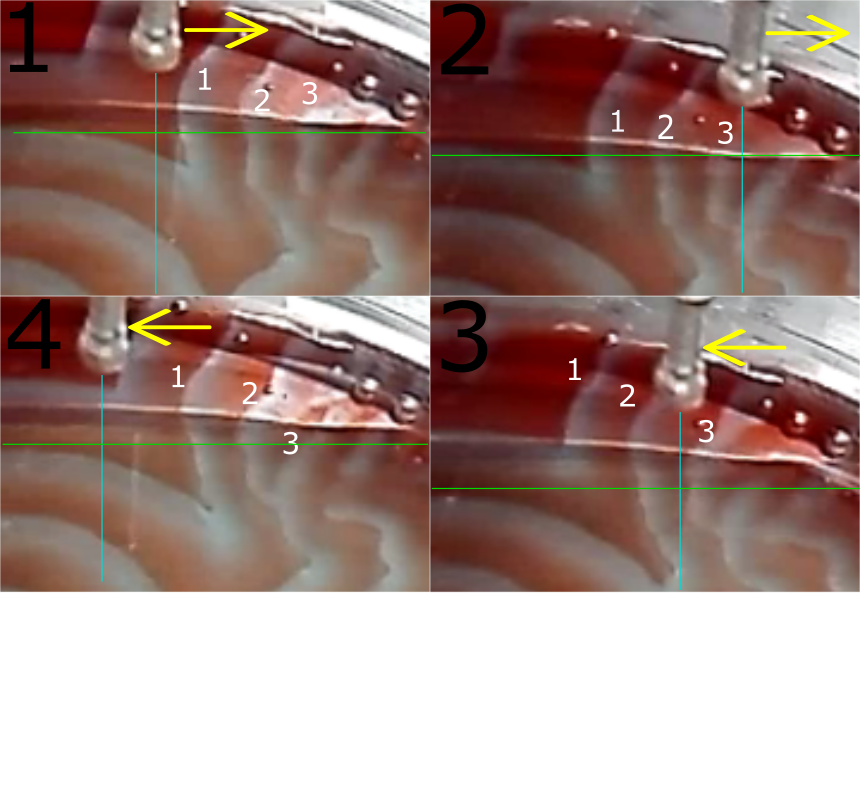
\includegraphics[width=0.8\textwidth]{img/secmkep.png}
\caption{Az ábrán a fekete nagy számok a mérés időbeli változását mutatják 1-4 sorrendben. A kis fehér számok a hullámok sorszámát mutatja. A vízszintes zöld vonal a pásztázás vonalát mutatja, a függőleges kék vonal az elektród test helyét mutatja. A zöld és a kék vonal keresztezésénel található az elektródtest vége, ami 1 $\upmu$-re merült a vizsgálandó BZ-reakcióelegybe. Szemmel látható, hogy az elektródtest nem okozott konvekcionális hatást a pásztázás során.}
\label{fig:secmkep}
\end{figure}

\begin{figure}
%% trim = top left bottom right
\centering
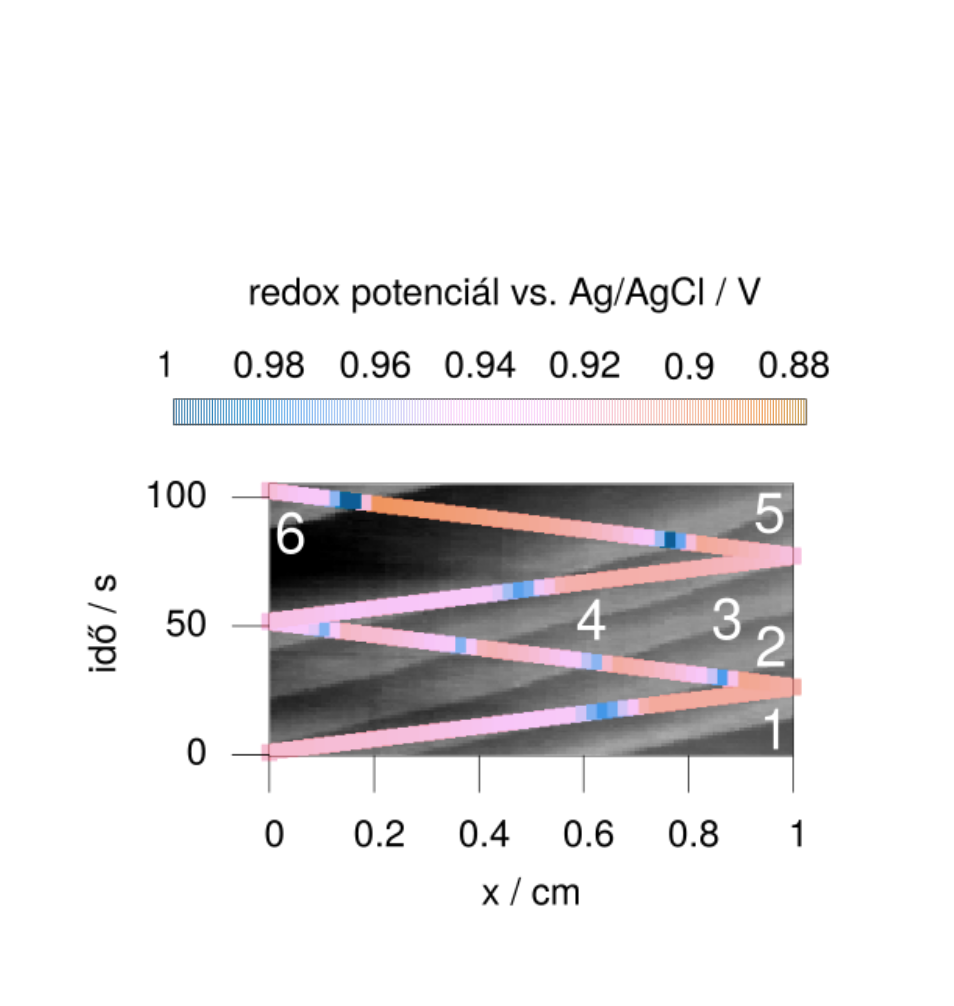
\includegraphics[width=0.8\textwidth]{img/spacetime2.eps}
\caption{ Az ábrán egy elektrokémiai tér-idő képet ábrazol egy optikai tér-idő képpel a háttérben. Az optikai tér-idő kép jobban látható, amennyiben előtte feltűntetjük az elektrokémiai információt. Az optikai képet az \emph{"Optikai tér-idő kép szerkeztése} című fejezetben leírt módszer alapján készítettem. Az ábrán látható világosabb csíkok a háttérben a BZ-reakció oxidációs hullámjait mutatja, amelyek a mikroelektródon éppen áthaladtak.
%Electrochemical space-time plot overlayed on top of the corresponding optical one.
%The potential of the carbon fiber microelectrode is shown as a function of spatiotemporal coordinates.
%Redox indicator was ferroin.
%The optical spatiotemporal image was grayscaled to allow better visibility when overlaying the electrochemical data.
%The brighter stripes correspond to the oxidizing waves.
%(B) The second scan cycle.
%Blue line: forward scan, red line: backwards scan.
%Note the shape of the peaks on the red curve, which is measured in the direction that is opposite to the chemical wave travel.
%The elongated portion of these peaks where the potential is decreasing, is not due to 
}
\label{fig:spatiotemporal}
\end{figure}
A \ref{fig:spatiotemporal} ábráról, valamint a készülék által rögzített koordináta, idő, potenciál adatokból meghatározhatjuk azon hullámok sebességét, melyeken a pásztázás során többször is adatot gyűjtöttünk. Ezeket az adatokat \ref{hullam} táblázatban foglaltam össze, és számítottam ki a hullámok terjedési sebességét.

\begin{table}[] 
\centering
\caption{\ref{fig:spatiotemporal} ábrán leolvasható a mérés során kapott elektrokémiai jel (kék elektrokémiai információ), a hozzá tartozó térkoordináta és idő adatok, valamint adat. Ennek segítségével különböző statisztikai adatok számíthatóak.}
\label{hullam}
\begin{tabular}{|c|c|c|c|c|}
\hline
\textbf{Hullám sorszáma} & \textbf{t (s)} & \textbf{E (mV)} & \textbf{x (mm)} & \textbf{v ($\upmu$m/s)}        \\ \hline
\multirow{2}{*}{2}       & 17             & 978             & 6,4             & \multirow{2}{*}{169,23} \\ \cline{2-4}
                         & 30             & 977             & 8,6             &                         \\ \hline
\multirow{3}{*}{5}       & 49             & 968             & 1               & \multirow{3}{*}{191,3}  \\ \cline{2-4}
                         & 64             & 975             & 4,8             &                         \\ \cline{2-4}
                         & 83,5           & 1027            & 7,6             &                         \\ \hline
\end{tabular}
\end{table}
